\section{Principal Component Analysis}



Since Coho were only found to be present in Stream BBB (Table~\ref{fig:kablemass} ), we investigate the environmental features that distinguish the streams from one another. Principal Component Analysis (`PCA') is a statistical technique that is used to study a dataset by reducing the number of dimensions. We use the R package `factoextra' \citep{facto} to compute the principal components of our stream data. PCA works by creating uncorrelated variables that maximize variance. The problem of finding principal components reduces to a simpler problem of solving an eigenvalue/eigenvector problem. PCA preserves much variance as possible while simultaneously providing uncorrelated variables to explain the variation in the data \citep{PCA}.

\vspace{5mm}

\begin{table}[H]
\begin{singlespace*}
\verbatiminput{Chapter5Images/pcaloadings.txt}
\end{singlespace*}
\caption{Coefficients from principal component analysis on Stream Data.}
\label{fig:pcaloadings}
\end{table}

Table ~\ref{fig:pcaloadings} is a table of direction vectors for our principal components.file:///C:/Users/User/Desktop/pcaloadings.txt

\begin{figure}[H]
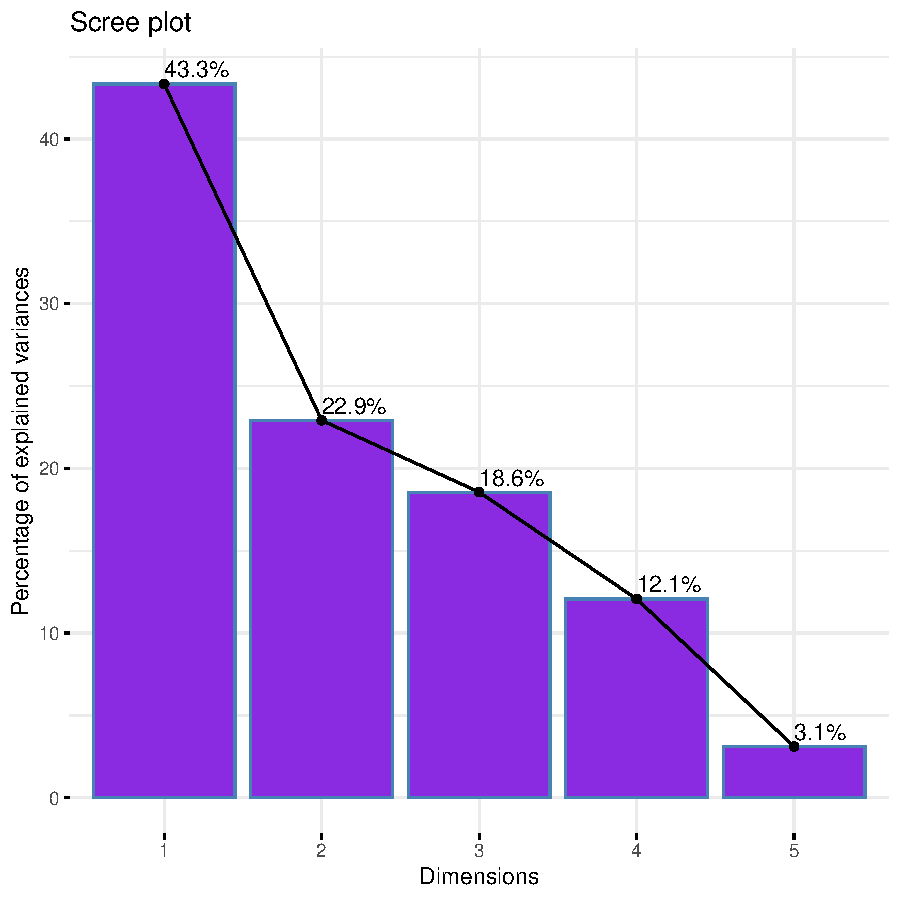
\includegraphics{Chapter5Images/scree.pdf}
\caption{Scree Plot for our principal component analysis.}
\label{fig:scree}
\end{figure}

Figure~\ref{fig:scree} is the Scree plot that summarizes the amount of variation explained by each principal component. The first two components alone explain more than 50\% of the variance in the dataset.

\begin{figure}[H]
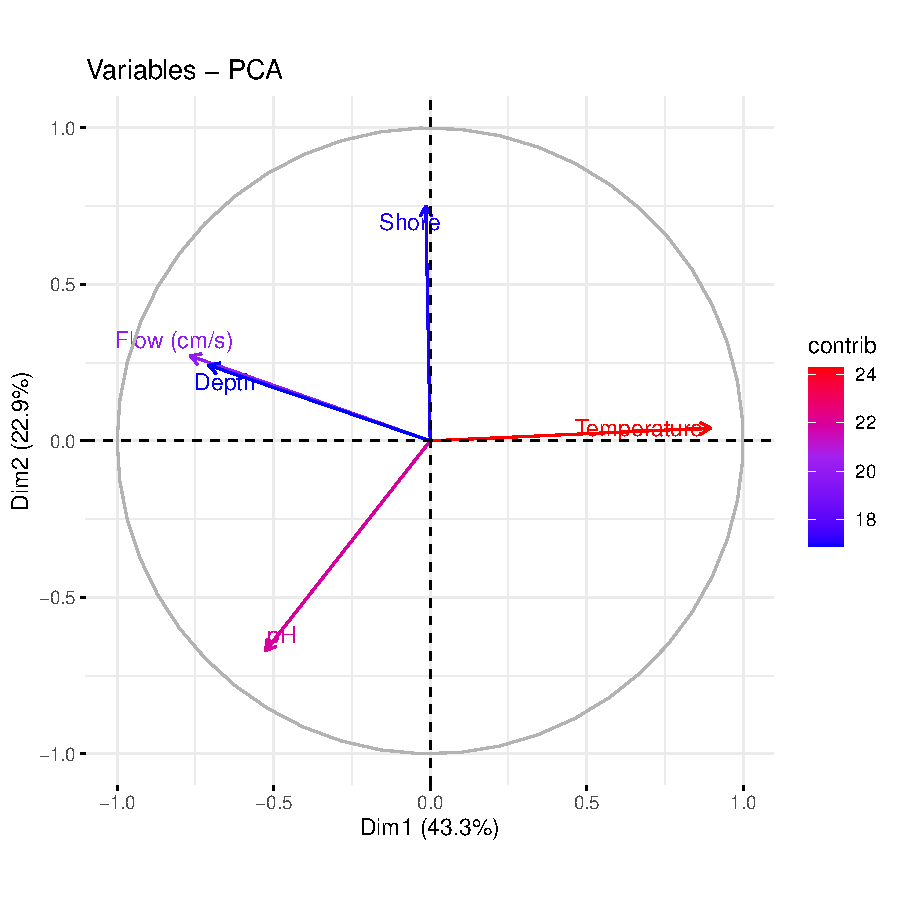
\includegraphics{Chapter5Images/pcaContrib.pdf}
\caption{Contributions of predictors towards explaining the variance. Note temperature and pH have particularly strong influence.}
\label{fig:pcacontrib}
\end{figure}

Figure~\ref{fig:pcacontrib} is a visualization of the contribution that each predictor has towards the principal components. Using the function prcomp and plotting gives us a way to visualize the dataset as projections on the principal components. From our visualization plot we can see that Temperature and pH have the greatest contributions to the first two dimensions.

\begin{figure}[H]
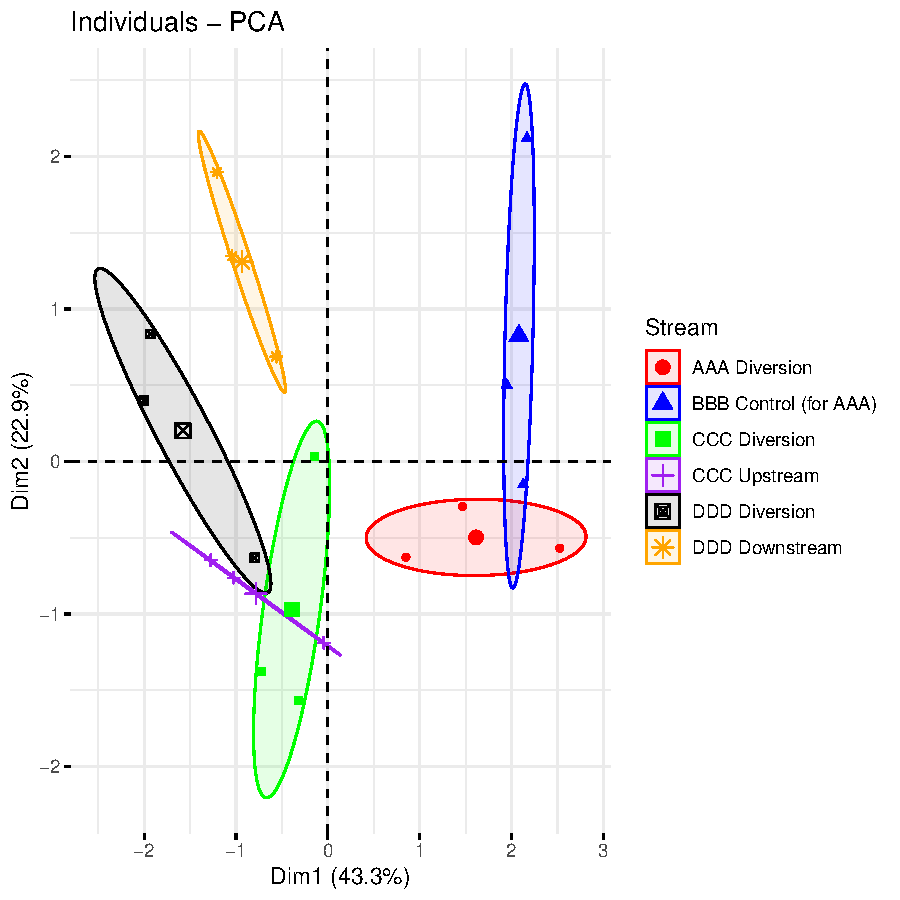
\includegraphics{Chapter5Images/streamPCA.pdf}
\caption{PCA on streams and reach. This visualization shows us which observations cluster eachother based off the first two principal components.}
\label{fig:pcastream}
\end{figure}

Figure ~\ref{fig:pcastream} is the result of applying PCA on the stream data, we can fit ellipsoids to each stream. As temperature has a large impact on the principal components, we see streams AAA and BBB separated from the other streams, and we can see they also have higher temperature compared to the other streams. pH also has a large contribution, with constant pH in stream CCC. This can be seen from the constant line that makes up CCC contribution. Note that Coho only appear in stream BBB which is significantly warmer than streams CCC and DDD.